\chapter {Resultado da Interface do Usuário}
\label{c:resultado_da_interface_do_usuario}

% ---
A Aplicação Web SIDE foi implantada em ambiente de produção, hospedada em um servidor conforme figura \ref{fig:servidor} na Escola de Engenharia Elétrica, Mecânica e de Computação da Universidade Federal de Goiás (EMC - UFG)\footnote{URL de Acesso ao SIDE: \url{http://200.137.220.157:8080/sideufg-front}}, possibilitando o cadastro de novos usuários que poderão fazer uso do sistema, acompanhando em tempo real as leituras de consumo e geração de todos os prédios da Universidade.

\begin{figure}[H]
    \centering
    \caption{ Servidor de Aplicação e unidades de armazenamento instalados na EMC.}
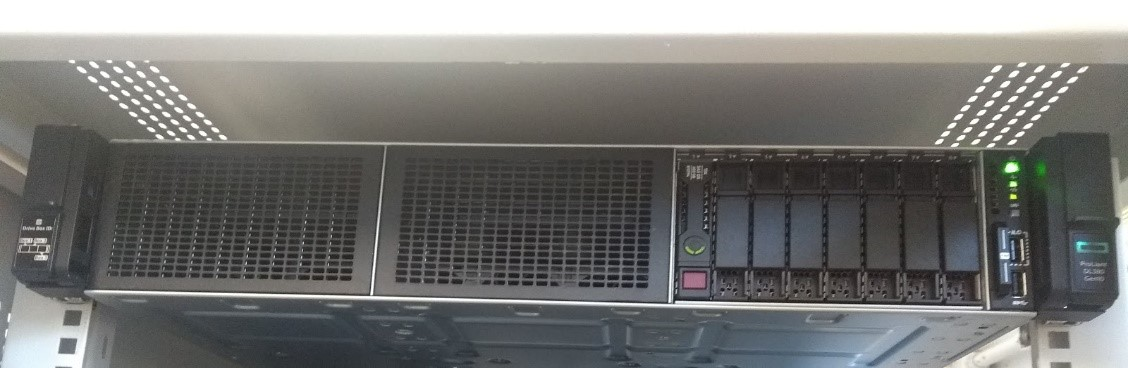
\includegraphics[width=\linewidth]{imagens/servidor.jpg}
    \caption*{Fonte: Próprio Autor}
    \label{fig:servidor}
\end{figure}

O desempenho do sistema permite acesso simultâneo por vários usuários mas caso seja necessário a aplicação pode ser replicada tanto o \textit{frontend} quanto o \textit{backend} de maneira separadas, facilitando a escalabilidade do sistema, através de contêineres Docker\footnote{Site da Plataforma Docker: \url{https://www.docker.com/}} por exemplo.